% vim: set spell spelllang=en tw=100 :

\documentclass[sigconf]{acmart}

\usepackage{amsmath}
\usepackage{amssymb}
\usepackage{cleveref}
\usepackage{tikz}

\usetikzlibrary{decorations, decorations.pathreplacing, calc, backgrounds}

\definecolor{uofgsandstone}{rgb}{0.321569, 0.278431, 0.231373}
\definecolor{uofglawn}{rgb}{0.517647, 0.741176, 0}
\definecolor{uofgcobalt}{rgb}{0, 0.615686, 0.92549}
\definecolor{uofgpumpkin}{rgb}{1.0, 0.72549, 0.282353}
\definecolor{uofgthistle}{rgb}{0.584314, 0.070588, 0.447059}

% cref style
\crefname{figure}{Figure}{Figures}
\Crefname{figure}{Figure}{Figures}

\newcommand{\citepos}[1]{\citet{#1}'s}

% pretty colours
\definecolor{uofgsandstone}{rgb}{0.321569, 0.278431, 0.231373}
\definecolor{magmapurple}{rgb}{0.505882, 0.145098, 0.505882}
\definecolor{magmaorange}{rgb}{0.984314, 0.529412, 0.380392}

% http://tex.stackexchange.com/questions/22100/the-bar-and-overline-commands
\newcommand{\shortoverline}[1]{\mkern 1.5mu\overline{\mkern-1.5mu#1\mkern-1.5mu}\mkern 1.5mu}

\newcommand*\samethanks[1][\value{footnote}]{\footnotemark[#1]}

% Copyright
%\setcopyright{none}
%\setcopyright{acmcopyright}
%\setcopyright{acmlicensed}
\setcopyright{rightsretained}
%\setcopyright{usgov}
%\setcopyright{usgovmixed}
%\setcopyright{cagov}
%\setcopyright{cagovmixed}


% DOI
\acmDOI{10.475/123_4}

% ISBN
\acmISBN{123-4567-24-567/08/06}

%Conference
\acmConference[$\textnormal{IA}^3$ 2017]{Seventh Workshop on Irregular Applications: Architectures and Algorithms}{November 2017}{Denver, Colorado USA}
\acmYear{2017}
\copyrightyear{2017}

\acmPrice{666.00}

\begin{document}
\title[Observations from Parallelising Three Subgraph Algorithms]{Observations from Parallelising Three Maximum Common (Connected) Subgraph Algorithms}
\titlenote{This work was supported by the Engineering and Physical Sciences
    Research Council [grant numbers EP/K503058/1, EP/M508056, and EP/P026842/1] and the ANR project
SoLStiCe (ANR-13-BS02-0002-01)}

\author{Ruth Hoffmann}
\affiliation{%
    \institution{University of St Andrews}
    \city{St Andrews, Scotland}
}

\author{Ciaran McCreesh}
\affiliation{%
    \institution{University of Glasgow}
    \city{Glasgow, Scotland}
}
\email{ciaran.mccreesh@glasgow.ac.uk}

\author{Samba Ndojh Ndiaye}
\affiliation{
    \institution{Universit\'e Lyon 1, LIRIS, UMR5205}
    \city{F-69621, France}
}

\author{Patrick Prosser}
\affiliation{%
    \institution{University of Glasgow}
    \city{Glasgow, Scotland}
}

\author{Craig Reilly}
\affiliation{%
    \institution{University of Glasgow}
    \city{Glasgow, Scotland}
}

\author{Christine Solnon}
\affiliation{
    \institution{INSA-Lyon, LIRIS, UMR5205}
    \city{F-69621, France}
}

\author{James Trimble}
\affiliation{%
    \institution{University of Glasgow}
    \city{Glasgow, Scotland}
}

% The default list of authors is too long for headers}
\renewcommand{\shortauthors}{R. Hoffmann et al.}

\begin{abstract}
    We discuss our experiences adapting three recent algorithms for maximum common (connected) subgraph
    problems to exploit multi-core parallelism. We consider the effects of different work
    distribution strategies and their interaction with value-ordering heuristics, and propose a
    search method which is risk-free, reproducible, and scalable, as well as beneficial. Our results
    show that each algorithm can be parallelised successfully using this strategy, with the
    multi-core algorithms we create being clearly better than the sequential ones. We then look in
    more detail at the results, on an instance by instance basis, and discuss how we should be
    measuring speedups for these kinds of algorithm.
\end{abstract}

\begin{CCSXML}
<ccs2012>
<concept>
<concept_id>10003752.10003809.10003716.10011136</concept_id>
<concept_desc>Theory of computation~Discrete optimization</concept_desc>
<concept_significance>500</concept_significance>
</concept>
<concept>
<concept_id>10003752.10003809.10010170</concept_id>
<concept_desc>Theory of computation~Parallel algorithms</concept_desc>
<concept_significance>500</concept_significance>
</concept>
<concept>
<concept_id>10003752.10003809.10011254.10011256</concept_id>
<concept_desc>Theory of computation~Branch-and-bound</concept_desc>
<concept_significance>500</concept_significance>
</concept>
<concept>
<concept_id>10003752.10003790.10003795</concept_id>
<concept_desc>Theory of computation~Constraint and logic programming</concept_desc>
<concept_significance>300</concept_significance>
</concept>
</ccs2012>
\end{CCSXML}

\ccsdesc[500]{Theory of computation~Discrete optimization}
\ccsdesc[500]{Theory of computation~Parallel algorithms}
\ccsdesc[500]{Theory of computation~Branch-and-bound}
\ccsdesc[300]{Theory of computation~Constraint and logic programming}

\keywords{Maximum common subgraph, Parallel branch and bound, Constraint programming}

\maketitle

\section{Introduction}

\begin{figure}[b]
    \centering
    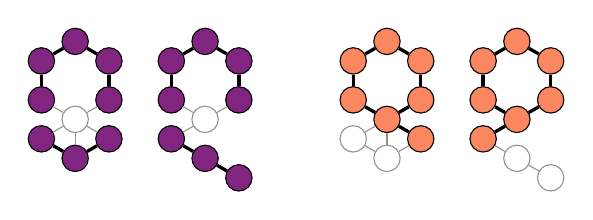
\begin{tikzpicture}[scale=0.33]%{{{
        \begin{scope}
            \node[draw, circle, fill=magmapurple, inner sep=0.5pt, font=\normalsize] (M1) at (90:1.5) {\phantom{0}};
            \node[draw, circle, fill=magmapurple, inner sep=0.5pt, font=\normalsize] (M2) at (150:1.5) {\phantom{0}};
            \node[draw, circle, fill=magmapurple, inner sep=0.5pt, font=\normalsize] (M3) at (30:1.5) {\phantom{0}};
            \node[draw, circle, fill=magmapurple, inner sep=0.5pt, font=\normalsize] (M4) at (210:1.5) {\phantom{0}};
            \node[draw, circle, fill=magmapurple, inner sep=0.5pt, font=\normalsize] (M5) at (330:1.5) {\phantom{0}};
            \node[draw, circle, draw=uofgsandstone!60, fill=white, inner sep=0.5pt, font=\normalsize] (M6) at (270:1.5) {\phantom{0}};
            \node[draw, circle, fill=magmapurple, inner sep=0.5pt, font=\normalsize] (M7) at ($(210:1.5) + (M6)$) {\phantom{0}};
            \node[draw, circle, fill=magmapurple, inner sep=0.5pt, font=\normalsize] (M8) at ($(330:1.5) + (M6)$) {\phantom{0}};
            \node[draw, circle, fill=magmapurple, inner sep=0.5pt, font=\normalsize] (M9) at ($(270:1.5) + (M6)$) {\phantom{0}};

            \draw [very thick] (M1) -- (M2);
            \draw [very thick] (M2) -- (M4);
            \draw [very thick] (M3) -- (M5);
            \draw [color=uofgsandstone!60] (M4) -- (M6);
            \draw [color=uofgsandstone!60] (M5) -- (M6);
            \draw [very thick] (M3) -- (M1);
            \draw [color=uofgsandstone!60] (M6) -- (M7);
            \draw [color=uofgsandstone!60] (M6) -- (M8);
            \draw [color=uofgsandstone!60] (M6) -- (M9);
            \draw [very thick] (M7) -- (M9);
            \draw [very thick] (M8) -- (M9);
        \end{scope}

        \begin{scope}[xshift=5cm]
            \node[draw, circle, fill=magmapurple, inner sep=0.5pt, font=\normalsize] (M1) at (90:1.5) {\phantom{0}};
            \node[draw, circle, fill=magmapurple, inner sep=0.5pt, font=\normalsize] (M2) at (150:1.5) {\phantom{0}};
            \node[draw, circle, fill=magmapurple, inner sep=0.5pt, font=\normalsize] (M3) at (30:1.5) {\phantom{0}};
            \node[draw, circle, fill=magmapurple, inner sep=0.5pt, font=\normalsize] (M4) at (210:1.5) {\phantom{0}};
            \node[draw, circle, fill=magmapurple, inner sep=0.5pt, font=\normalsize] (M5) at (330:1.5) {\phantom{0}};
            \node[draw, circle, draw=uofgsandstone!60, fill=white, inner sep=0.5pt, font=\normalsize] (M6) at (270:1.5) {\phantom{0}};
            \node[draw, circle, fill=magmapurple, inner sep=0.5pt, font=\normalsize] (M7) at ($(210:1.5) + (M6)$) {\phantom{0}};
            \node[draw, circle, fill=magmapurple, inner sep=0.5pt, font=\normalsize] (M8) at ($(270:1.5) + (M6)$) {\phantom{0}};
            \node[draw, circle, fill=magmapurple, inner sep=0.5pt, font=\normalsize] (M9) at ($(330:1.5) + (M8)$) {\phantom{0}};

            \draw [very thick] (M1) -- (M2);
            \draw [very thick] (M2) -- (M4);
            \draw [very thick] (M3) -- (M5);
            \draw [color=uofgsandstone!60] (M4) -- (M6);
            \draw [color=uofgsandstone!60] (M5) -- (M6);
            \draw [very thick] (M3) -- (M1);
            \draw [color=uofgsandstone!60] (M6) -- (M7);
            \draw [very thick] (M7) -- (M8);
            \draw [very thick] (M8) -- (M9);
        \end{scope}

        \begin{scope}[xshift=12cm]
            \node[draw, circle, fill=magmaorange, inner sep=0.5pt, font=\normalsize] (M1) at (90:1.5) {\phantom{0}};
            \node[draw, circle, fill=magmaorange, inner sep=0.5pt, font=\normalsize] (M2) at (150:1.5) {\phantom{0}};
            \node[draw, circle, fill=magmaorange, inner sep=0.5pt, font=\normalsize] (M3) at (30:1.5) {\phantom{0}};
            \node[draw, circle, fill=magmaorange, inner sep=0.5pt, font=\normalsize] (M4) at (210:1.5) {\phantom{0}};
            \node[draw, circle, fill=magmaorange, inner sep=0.5pt, font=\normalsize] (M5) at (330:1.5) {\phantom{0}};
            \node[draw, circle, fill=magmaorange, inner sep=0.5pt, font=\normalsize] (M6) at (270:1.5) {\phantom{0}};
            \node[draw, circle, draw=uofgsandstone!60, fill=white, inner sep=0.5pt, font=\normalsize] (M7) at ($(210:1.5) + (M6)$) {\phantom{0}};
            \node[draw, circle, fill=magmaorange, inner sep=0.5pt, font=\normalsize] (M8) at ($(330:1.5) + (M6)$) {\phantom{0}};
            \node[draw, circle, draw=uofgsandstone!60, fill=white, inner sep=0.5pt, font=\normalsize] (M9) at ($(270:1.5) + (M6)$) {\phantom{0}};

            \draw [very thick] (M1) -- (M2);
            \draw [very thick] (M2) -- (M4);
            \draw [very thick] (M3) -- (M5);
            \draw [very thick] (M4) -- (M6);
            \draw [very thick] (M5) -- (M6);
            \draw [very thick] (M3) -- (M1);
            \draw [color=uofgsandstone!60] (M6) -- (M7);
            \draw [very thick] (M6) -- (M8);
            \draw [color=uofgsandstone!60] (M6) -- (M9);
            \draw [color=uofgsandstone!60] (M7) -- (M9);
            \draw [color=uofgsandstone!60] (M8) -- (M9);
        \end{scope}

        \begin{scope}[xshift=17cm]
            \node[draw, circle, fill=magmaorange, inner sep=0.5pt, font=\normalsize] (M1) at (90:1.5) {\phantom{0}};
            \node[draw, circle, fill=magmaorange, inner sep=0.5pt, font=\normalsize] (M2) at (150:1.5) {\phantom{0}};
            \node[draw, circle, fill=magmaorange, inner sep=0.5pt, font=\normalsize] (M3) at (30:1.5) {\phantom{0}};
            \node[draw, circle, fill=magmaorange, inner sep=0.5pt, font=\normalsize] (M4) at (210:1.5) {\phantom{0}};
            \node[draw, circle, fill=magmaorange, inner sep=0.5pt, font=\normalsize] (M5) at (330:1.5) {\phantom{0}};
            \node[draw, circle, fill=magmaorange, inner sep=0.5pt, font=\normalsize] (M6) at (270:1.5) {\phantom{0}};
            \node[draw, circle, fill=magmaorange, inner sep=0.5pt, font=\normalsize] (M7) at ($(210:1.5) + (M6)$) {\phantom{0}};
            \node[draw, circle, draw=uofgsandstone!60, fill=white, inner sep=0.5pt, font=\normalsize] (M8) at ($(270:1.5) + (M6)$) {\phantom{0}};
            \node[draw, circle, draw=uofgsandstone!60, fill=white, inner sep=0.5pt, font=\normalsize] (M9) at ($(330:1.5) + (M8)$) {\phantom{0}};

            \draw [very thick] (M1) -- (M2);
            \draw [very thick] (M2) -- (M4);
            \draw [very thick] (M3) -- (M5);
            \draw [very thick] (M4) -- (M6);
            \draw [very thick] (M5) -- (M6);
            \draw [very thick] (M3) -- (M1);
            \draw [very thick] (M6) -- (M7);
            \draw [draw=uofgsandstone!60] (M7) -- (M8);
            \draw [draw=uofgsandstone!60] (M8) -- (M9);
        \end{scope}
\end{tikzpicture}
\caption{A maximum common subgraph of the first two graphs has eight vertices, shaded. A maximum
common \emph{connected} subgraph, shown on the right, has only seven vertices.}
\label{figure:mcsexample}
\end{figure}

A \emph{subgraph isomorphism} is an injective mapping from a \emph{pattern} graph to a \emph{target}
graph which maps adjacent vertices to adjacent vertices---that is, it \emph{preserves adjacency}. It
is \emph{induced} if additionally it maps non-adjacent vertices to non-adjacent vertices, preserving
non-adjacency. When working with labelled graphs, a subgraph isomorphism must preserve labels, and
on directed graphs, it must preserve orientation. A \emph{common induced subgraph} of two graphs $G$
and $H$ is a pair of induced subgraph isomorphisms from a pattern graph $P$, one to $G$ and one to
$H$. A \emph{maximum common induced subgraph} is one with as many vertices as possible.

Finding a maximum common subgraph is the key step in measuring the similarity or difference between
two graphs \citep{DBLP:journals/prl/Bunke97,DBLP:journals/prl/FernandezV01,o:Kriege15}: to determine
the difference between two graphs, we find what they have in common, and then take everything left
over. Because of this, maximum common subgraph problems frequently arise in biology and chemistry
\citep{DBLP:journals/jcamd/RaymondW02a,o:EhrlichR11,DBLP:journals/dam/GayFMSS14} where graphs
represent molecules, but also in applications including computer vision
\citep{DBLP:journals/jair/CookH94,DBLP:conf/gbrpr/CombierDS13}, computer-aided manufacturing
\citep{o:LuoWSN17}, crisis management \citep{o:DelavalladeFLL16}, deanonymising datasets
\citep{o:SharadD13}, the analysis of source code \citep{DBLP:journals/tkde/DjokoCH97}, binary
programs \citep{DBLP:conf/icics/GaoRS08}, and circuit designs \citep{DBLP:journals/jair/CookH94}, in
malware detection \citep{DBLP:journals/compsec/ParkRS13}, social network analysis
\citep{DBLP:journals/tkde/FangYZZ15}, graph database query explanations
\citep{DBLP:journals/jcss/VasilyevaTBL16}, and in character recognition problems
\citep{DBLP:journals/pr/LuRS91}.  A common variant of the problem requires a largest
\emph{connected} subgraph
\citep{DBLP:journals/tcs/Koch01,DBLP:journals/jcamd/RaymondW02a,DBLP:conf/mco/VismaraV08,o:EhrlichR11,o:LuoWSN17}.
As illustrated in \cref{figure:mcsexample}, the maximum common connected subgraph cannot be deduced
from the maximum common subgraph.

Although both variants are NP-hard, some progress has been made towards solving the problem in
practice.  This paper looks at three recent branch and bound algorithms for maximum common
(connected) induced subgraph problems, each of which is the state of the art for certain classes of
instance. We discuss our experiences in adding parallel tree-search to these three algorithms. In
each case, our results show that the parallel version of the algorithm is clearly better than the
sequential version, although a closer look at the results shows many nuances.

\section{Sequential Algorithms}

\subsection{Encoding as Maximum Clique}

\subsection{Constraint Programming}

The maximum common subgraph problem may be reformulated as a constraint optimisation problem, as
follows.  Observe that an equivalent definition of a common subgraph of graphs $G$ and $H$ is an
injective partial mapping from $G$ to $H$ which preserves both adjacency and non-adjacency. Hence we
pick whichever input graph has fewer vertices, and call it the \emph{pattern}; the other graph is
called the \emph{target}. The model is then to construct an injective, partial mapping from the
pattern to the target, preserving both adjacency and non-adjacency. Thus, for each vertex in the
pattern, we create a variable, whose domain ranges over each vertex in the target graph, plus an
additional value $\bot$. We then have three sets of constraints. The first set says that for each
pair of adjacent vertices in the pattern (that is, for each edge in the pattern), if neither of
these vertices are mapped to $\bot$ then these vertices must be mapped to an adjacent pair of target
vertices. The second set is similar, but looks at non-adjacent pairs (or non-edges).  Finally, the
third set ensures injectivity, by enforcing that the variables must be all different except when
using $\bot$.

?? Either by binary constraints between all pairs, or a specialised propagator.

?? Objective.

?? One approach is branch and bound search over this model. Pick a variable, ... . cite.

?? Ensuring connectedness

\subsection{Domain Splitting}

Due to the special structure of the maximum common subgraph problem, the following property holds
throughout the search process using the CP model: any two variables either have domains with no
values in common (with the possible exception of $\bot$), or have identical domains. The algorithm
McSplit exploits this property, while exploring essentially the same search tree as the CP model.
Rather than storing a domain for each vertex in $\operatorname{V}(G)$, which results in redundant
storage in cases where domains are identical, equivalence classes of vertices in
$\operatorname{V}(G)$ are stored, and a set of candidate vertices in $H$ is maintained for each
equivalence class. This enables fast propagation of the constraints and smaller memory requirements.
In addition, the data structure enables good branching heuristics to be calculated cheaply.

\subsection{$k$-less Subgraph Isomorphism}

The algorithm as described by Hoffmann, McCreesh, and Reilly \cite{DBLP:conf/aaai/HoffmannMR17} approaches the subgraph isomorphism problem by asking the question ``if a pattern graph cannot be found in the target, how much of the pattern graph can be found?''. The $k{\downarrow}$ algorithm tries to solve the subgraph isomorphism problem first for $k=0$ (the whole pattern graph can be found in the target), should that be not satisfiable, it tries to solve the problem for $k=1$ (one vertex cannot be matched) should that also not be satisfiable, it iterates $k$ further by a small number to keep the shrinking pattern graph within a reasonable size. By unmatching some vertices  invariants are weakened but kept effective. Specifically, invariants based around paths and degrees of vertices hold.

This technique bridges the subgraph isomorphism problem with the maximal common subgraph problem. The iteration of the decision problem (iterating over $k$) leads to an algorithm with rivalling runtimes.

\section{Parallel Search}

?? Approach

\section{Empirical Evaluation}

We perform our experiments on systems with dual Intel Xeon E5-2640 v2 processors and 64GBytes RAM,
running Ubuntu 14.04, with GCC 5.3.0 as the compiler. Each machine has a total of sixteen cores, and
hyper-threading is enabled, so we run experiments with 32 threads except where otherwise noted.
Most of our instances come from a standard benchmark set
\citep{DBLP:journals/prl/SantoFSV03,DBLP:journals/jgaa/ConteFV07} for maximum common subgraph
problems.  This benchmark set can be used in a number of ways, for different variants of the
problem. We use it to create five families of instance, as follows:

\begin{description}
    \item[Unlabelled] instances, by selecting the first ten members of each parameter class where the
        graphs have up to 50 vertices each---this gives us a total of 4,110 instances.

    \item[Vertex labelled] instances, by selecting the first ten members of each parameter class
        (and so graphs have up to 100 vertices each), applying the 33\% labelling scheme for
        vertices only, and treating edges as undirected. This gives 8,140 instances.

    \item[Both labelled, directed] instances, by selecting the first ten members of each parameter
        class, and applying the 33\% labelling scheme to both vertices and edges. Again, this gives
        8,140 instances.

    \item[Unlabelled, connected] instances, using the same instances as the \emph{unlabelled} case.

    \item[Both labelled, connected] instances, starting in the same way as the \emph{both labelled,
        directed} case. These are then converted to undirected graphs by treating edges as
        undirected, picking the label of the lower-numbered edge.
\end{description}

\noindent
Following \citet{DBLP:conf/aaai/HoffmannMR17}, we also work with the 5,725 \textbf{Large} instances
originally used for studying portfolios of subgraph isomorphism algorithms
\citep{DBLP:conf/lion/KotthoffMS16}. These graphs are unlabelled and undirected, and can include up
to 6,671 vertices. We do not use the clique encoding on these instances due to its impractical
memory requirements for large graphs.

\subsection{Parallel Search is Better Overall}

\begin{figure*}[tb]
    \includegraphics*{gen-graph-cumulative-plain.pdf}
    \hfill
    \includegraphics*{gen-graph-cumulative-33v.pdf}
    \hfill
    \includegraphics*{gen-graph-cumulative-33ved.pdf}

    \vspace*{1em}

    \includegraphics*{gen-graph-cumulative-plain-connected.pdf}
    \hfill
    \includegraphics*{gen-graph-cumulative-33ve-connected.pdf}
    \hfill
    \includegraphics*{gen-graph-cumulative-sip.pdf}

    \caption{The cumulative number of instances solved over time, for different families and
    algorithms. The 32 threaded parallel versions (shown using dotted lines) are always better in
aggregate than the sequential versions (shown using solid lines).}\label{figure:cumulative}
\end{figure*}

In \cref{figure:cumulative} we plot empirical cumulative distribution functions showing the number
of instances solved over time, for both sequential (solid lines) and parallel (dotted lines)
versions of each algorithm.  Cumulative plots are commonly used in constraint programming and
boolean satisfiability for comparing aggregate behaviour of solvers (sometimes with the axes
reversed, in which case they are called \emph{cactus} plots).  To read these plots, make a choice of
timeout along the $x$-axis, which uses a log scale. The $y$ value at that point shows the number of
instances whose runtime (individually) is at most $x$, for a particular algorithm. In other words,
at any given $x$ value, the highest line shows which algorithm is able to solve the largest number
of instances using a per-instance timeout of that $x$ value, bearing in mind that the actual sets of
instances solved by each algorithm may be completely different.

Each plot gives the same conclusion: if we are working with a timeout of at least $10^2$
milliseconds, then for any problem family and any sequential algorithm, if given the option of
switching to the corresponding parallel algorithm, then we should do so.

\subsection{A Closer Look at Clique}

\begin{figure*}[tb]
    \includegraphics*{gen-graph-scatter-plain-clique-vs-clique-par-t32.pdf}
    \hfill
    \includegraphics*{gen-graph-scatter-33v-clique-vs-clique-par-t32.pdf}
    \hfill
    \includegraphics*{gen-graph-scatter-33ved-clique-vs-clique-par-t32.pdf}
    \hfill
    \includegraphics*{gen-graph-scatter-plain-connected-clique-vs-clique-par-t32.pdf}
    \hfill
    \includegraphics*{gen-graph-scatter-33ve-connected-clique-vs-clique-par-t32.pdf}

    \vspace*{1em}

    \includegraphics*{gen-graph-histogram-plain-clique-vs-clique-par-t32.pdf}
    \hfill
    \includegraphics*{gen-graph-histogram-33v-clique-vs-clique-par-t32.pdf}
    \hfill
    \includegraphics*{gen-graph-histogram-33ved-clique-vs-clique-par-t32.pdf}
    \hfill
    \includegraphics*{gen-graph-histogram-plain-connected-clique-vs-clique-par-t32.pdf}
    \hfill
    \includegraphics*{gen-graph-histogram-33ve-connected-clique-vs-clique-par-t32.pdf}

    \caption{On the top row, per-instance speedups, using the clique algorithm. The $x$-axis is
    sequential performance and the $y$-axis is 32 threaded performance, so points below the diagonal
    line represent a speedup. Darker points represent instances where the solution is relatively
    large compared to the order of the input graphs. Below, histograms plotting the distribution of
    speedups for instances whose sequential runtime was at least 500 milliseconds, and below the
    timeout.}
\end{figure*}

\begin{figure}[tb]
    \includegraphics{gen-graph-as-clique.pdf}

    \caption{Aggregate speedups from the clique algorithm using 32 threads, for each supported
    family of instances.}
\end{figure}

% \begin{figure*}[tb]
%     \includegraphics*{gen-graph-scatter-plain-clique-vs-clique-par-t32.pdf}
%     \hfill
%     \includegraphics*{gen-graph-scatter-plain-kdown-vs-kdown-par-t32.pdf}
%     \hfill
%     \includegraphics*{gen-graph-scatter-plain-mcsplit-vs-mcsplit-par-t32.pdf}
%     \hfill
%     \includegraphics*{gen-graph-scatter-33v-clique-vs-clique-par-t32.pdf}
%     \hfill
%     \includegraphics*{gen-graph-scatter-33v-mcsplit-vs-mcsplit-par-t32.pdf}
% 
%     \vspace*{1em}
% 
%     \includegraphics*{gen-graph-scatter-33ved-clique-vs-clique-par-t32.pdf}
%     \hfill
%     \includegraphics*{gen-graph-scatter-33ved-mcsplit-vs-mcsplit-par-t32.pdf}
%     \hfill
%     \includegraphics*{gen-graph-scatter-sip-kdown-vs-kdown-par-t32.pdf}
%     \hfill
%     \includegraphics*{gen-graph-scatter-sip-mcsplit-vs-mcsplit-par-t32.pdf}
% 
%     \caption{Per-instance speedups. The $x$-axis is sequential performance and the $y$-axis is 32
%     threaded performance, so points below the diagonal line represent a speedup.}
% \end{figure*}
% 
\begin{figure}[tb]
    \includegraphics*{gen-graph-scatter-33ved-clique-vs-clique-par-t2.pdf}
    \hfill
    \includegraphics*{gen-graph-scatter-33ved-clique-par-t2-vs-clique-par-t4.pdf}

    \vspace*{1em}

    \includegraphics*{gen-graph-scatter-33ved-clique-par-t4-vs-clique-par-t8.pdf}
    \hfill
    \includegraphics*{gen-graph-scatter-33ved-clique-par-t8-vs-clique-par-t16.pdf}

    \vspace*{1em}

    \includegraphics*{gen-graph-scatter-33ved-clique-par-t16-vs-clique-par-t32.pdf}
    \hfill
    \includegraphics*{gen-graph-scatter-33ved-clique-par-t32r-vs-clique-par-t32.pdf}

    \caption{Per-instance speedups from the clique algorithm on vertex- and edge-labelled, directed
    instances, when going from sequential to two threads in the first plot, then increasing the
    number of threads in subsequent plots. The final plot shows 32 threads versus a repeated run
    also with 32 threads.}
\end{figure}
% 
% \begin{figure}[tb]
%     \includegraphics*{gen-graph-scatter-33ved-clique-cilk-t32r-vs-clique-cilk-t32.pdf}
%     \hfill
%     \includegraphics*{gen-graph-scatter-33ved-clique-vs-clique-cilk-t2.pdf}
% 
%     \vspace*{1em}
% 
%     \includegraphics*{gen-graph-scatter-33ved-clique-cilk-t2-vs-clique-cilk-t4.pdf}
%     \hfill
%     \includegraphics*{gen-graph-scatter-33ved-clique-cilk-t4-vs-clique-cilk-t8.pdf}
% 
%     \vspace*{1em}
% 
%     \includegraphics*{gen-graph-scatter-33ved-clique-cilk-t8-vs-clique-cilk-t16.pdf}
%     \hfill
%     \includegraphics*{gen-graph-scatter-33ved-clique-cilk-t16-vs-clique-cilk-t32.pdf}
% 
%     \caption{Scalability and reproducibility, clique algorithm, Cilk.}
% \end{figure}
% 
% \begin{figure}[tb]
%     \includegraphics*{gen-graph-scatter-plain-mcsplit-par-t32r-vs-mcsplit-par-t32.pdf}
%     \hfill
%     \includegraphics*{gen-graph-scatter-plain-mcsplit-vs-mcsplit-par-t2.pdf}
% 
%     \vspace*{1em}
% 
%     \includegraphics*{gen-graph-scatter-plain-mcsplit-par-t2-vs-mcsplit-par-t4.pdf}
%     \hfill
%     \includegraphics*{gen-graph-scatter-plain-mcsplit-par-t4-vs-mcsplit-par-t8.pdf}
% 
%     \vspace*{1em}
% 
%     \includegraphics*{gen-graph-scatter-plain-mcsplit-par-t8-vs-mcsplit-par-t16.pdf}
%     \hfill
%     \includegraphics*{gen-graph-scatter-plain-mcsplit-par-t16-vs-mcsplit-par-t32.pdf}
% 
%     \caption{Scalability and reproducibility, McSplit algorithm.}
% \end{figure}

\subsection{A Closer Look at $k{\downarrow}$}

\begin{figure}[tb]
    \includegraphics*{gen-graph-scatter-plain-kdown-vs-kdown-par-t32.pdf}
    \hfill
    \includegraphics*{gen-graph-scatter-sip-kdown-vs-kdown-par-t32.pdf}

    \vspace*{1em}

    \includegraphics{gen-graph-as-kdown.pdf}

    \caption{On the top row, per-instance speedups, using the $k{\downarrow}$ algorithm. The
    $x$-axis is sequential performance and the $y$-axis is 32 threaded performance. Below,
    aggregate speedups for both families.}
\end{figure}

\begin{figure}[tb]
    \includegraphics*{gen-graph-scatter-plain-kdown-par-t4-vs-kdown-par-t16.pdf}
    \hfill
    \includegraphics*{gen-graph-scatter-plain-kdown-par-t32r-vs-kdown-par-t32.pdf}

    \caption{Scalability and reproducibility of the $k{\downarrow}$ algorithm.}
\end{figure}

\subsection{A Closer Look at McSplit}

\begin{figure}[tb]
    \includegraphics*{gen-graph-scatter-plain-mcsplit-vs-mcsplit-par-t32.pdf}
    \hfill
    \includegraphics*{gen-graph-scatter-33v-mcsplit-vs-mcsplit-par-t32.pdf}

    \vspace*{1em}

    \includegraphics*{gen-graph-scatter-33ved-mcsplit-vs-mcsplit-par-t32.pdf}
    \hfill
    \includegraphics*{gen-graph-scatter-plain-connected-mcsplit-vs-mcsplit-par-t32.pdf}

    \vspace*{1em}

    \includegraphics*{gen-graph-scatter-33ve-connected-mcsplit-vs-mcsplit-par-t32.pdf}
    \hfill
    \includegraphics*{gen-graph-scatter-sip-mcsplit-vs-mcsplit-par-t32.pdf}

    \vspace*{1em}

    \includegraphics{gen-graph-as-mcsplit.pdf}

    \caption{On the top three rows, per-instance speedups, using the splitting algorithm. The
    $x$-axis is sequential performance and the $y$-axis is 32 threaded performance. On the final
    row, aggregate speedups for both families.}
\end{figure}

\begin{figure}[tb]
    \includegraphics*{gen-graph-scatter-plain-mcsplit-par-t4-vs-mcsplit-par-t16.pdf}
    \hfill
    \includegraphics*{gen-graph-scatter-plain-mcsplit-par-t32r-vs-mcsplit-par-t32.pdf}

    \caption{Scalability and reproducibility of the splitting algorithm.}
\end{figure}

\subsection{Old Text}

Cumulative performance plots comparing each parallel algorithm to its sequential version are given
in ??, using 32 threads on 16 core hyper-threaded Intel Xeon
E5-2640 v2 systems. The results are consistent: in each case the parallel algorithm is clearly and
substantially better than its sequential version, except when the sequential runtime is below 100
milliseconds.

?? gives instance-by-instance comparisons for a representative subset of
these algorithm and problem combinations. For the clique algorithm on unlabelled graphs (top left),
the results show fairly consistent speedups for harder instances: there is only a single instance
whose sequential runtime is over two seconds where we obtain a speedup of less than ten. We also see
a significant number of superlinear speedups. This is because there are relatively long proofs of
optimality for most of the harder instances, but strong solutions are usually found quickly (and
where they are not, the additional diversity helps). The results are similarly positive on
labelled graphs (centre left), with speedups of greater than ten being the norm for harder
instances, although there is more variety in the results.

For $k{\downarrow}$ on the unlabelled maximum common subgraph instances (top centre), the typical speedup
is between two and ten, and occasionally there are speedups of between ten and one hundred. A few
instances show small slowdowns: remember that when running 32 threads on a 16 core, hyper-threaded
system, each individual thread runs somewhat slower than it would if only a single thread were
running---in other words, these slight slowdowns are due to hardware effects, not changes to the
search tree.

On the larger subgraph isomorphism instances (bottom left), we see a concentration of speedups
of around ten. We also see strongly superlinear speedups in some cases, with eight
instances finishing in under one second which timed out sequentially at one thousand seconds.
Examining these instances closely shows that in each case, they are satisfiable with either $k = 0$
or very low values of $k$, and that the superlinear speedups are due to the parallel search
introducing early diversity, offsetting an incorrect initial value-ordering heuristic choice. We
also see more instances with slight absolute slowdowns: these are instances where the additional
threads contribute no helpful work to the solution, and where the slowdown due to not having 32
times as many resources when using 32 threads is particularly pronounced (memory contention is much
more of a problem for these larger graphs). Although not ideal, in aggregate these results are rare
and are more than offset by the superlinear speedups for other instances.

What about the splitting algorithm? On unlabelled instances (top right), our speedups are typically
between those obtained from the clique algorithm and those from $k{\downarrow}$, being mainly a
little below ten times. However, in some cases we see absolute slowdowns of up to four times: in
these cases, parallelism does little, and is not enough to offset the costs we paid when switching
from an in-place data structure to a data structure which requires copying. Interestingly, we also
see many more superlinear speedups for this algorithm, which suggests that its value ordering
heuristics are particularly poor early-on in search. (This last point is not particularly
surprising: compared to $k{\downarrow}$, the splitting algorithm does not try to reduce domains at
all at the top of search. The clique encoding, meanwhile, is able to capture even richer information
about variable-value relationships. The splitting algorithm is fast, but comparatively stupid.)

Similar trends occur with the subgraph isomorphism instances (bottom right), and the absolute
slowdowns go as high as a factor of ten---this is on instances with particularly large
target graphs, where copying is most expensive, and where there is a high branching factor at the
root of the search tree. Again, superlinear speedups are common.

On labelled instances (centre right), the parallel performance is less erratic. Although we no
longer see absolute slowdowns (excluding on very easy instances), we also see fewer superlinear
speedups, with most speedups being between one and ten. In many of these instances, parallelism
does very little: restricting splitting to a depth of five in these cases gives work balance
problems, but does help us avoid the substantial overheads that come with deeper splitting. This is
because the search trees for these instances tend to have a very low branching factor---in
constraint programming terms, the labels make each domain contain only a few values.

?? show that for all three
algorithms, parallel search is beneficial, and also (reasonably) risk-free: although in a few cases the
constant factor slowdowns due to hardware limitations and having to make changes to data structures
are unpleasant, we do not encounter any exponential slowdowns due to search tree changes. But what
about reproducibility and scalability? Further experiments in ??
establish that both of these properties also hold. In the left-hand column, we plot each algorithm
run against itself, using 32 threads in both cases. For the clique and $k{\downarrow}$ approaches,
every instance is on the central diagonal line, showing an extremely high level of reproducibility.
For the splitting algorithm, there is a little more variability, particularly for easier instances:
inspecting the results suggests that this is not down to different amounts of search work being
performed, but rather whether or not helper threads end up triggering additional copying.

In the right-hand column of ??, we plot the effects of moving from 8
threads (on the same system) to 32 threads. Points below the diagonal line indicate an improvement.
For the clique approach, increasing the number of threads is unequivocally beneficial. For the
$k{\downarrow}$ algorithm, the benefits are slim, and sometimes performance worsens slightly due to
memory contention (not work done) but we do not see any exponential slowdowns. Finally, for the
splitting algorithm, the results are usually strictly better, although in a few cases the overheads
increase further giving a slowdown; we also see an increase in the occurrence of strongly
superlinear speedups.

It is likely that the parallel results for the splitting algorithm can be improved further. In the
labelled case, we are often not obtaining a good work balance. However, deeper splitting is
expensive, particularly with larger graphs. One option to consider would be recomputing parts of the
search tree to avoid the costs of potentially allowing a copy in the future. This would be extremely
unpleasant from an implementation perspective, but may be necessary to obtain more even results.
However, even without this change, the parallel algorithm is clearly preferable to the sequential
one.

\section{Conclusion}

\bibliographystyle{ACM-Reference-Format}
\bibliography{combined}

\end{document}
